\epigraph{Not all those who wander are lost}
{\textit{J.R.R. Tolkien}}

\section{Transition from Familiar Problems}

Most problems you have probably met before come with some kind of scaffolding.

In mathematics, you are given an equation and expected to apply a known method. In physics, you identify the model, plug in the numbers, and hope the units work out in your favour. Even when a problem is difficult, there is usually a sense of what kind of solution it requires. You may not immediately know how to proceed, but you recognise the structure of the task. You know what tools are available, what progress might look like, and roughly how far you are from an answer.

\section{Why Codebreaking Feels Different}

Codebreaking does not usually begin with that same clarity.

When you first encounter a difficult cipher, nobody hands you a tidy label saying this is a \texttt{substitution cipher} or this one is \texttt{Vigenère but with a twist}\footnote{I must say this isn't strictly true. Depending on how generous Harry and Jodie are feeling, they might let a small hint or two slip before the first deadline!}. There is no signpost telling you whether the symbols represent letters, groups of letters, sounds, numbers, or something much weirder.

Instead of being guided towards a method, you are presented with something that has been deliberately designed to conceal its structure, so you have to work out what the problem even is before you can begin solving it. This is, unfortunately, much less glamorous than it sounds and often involves staring at repeated symbols until your brain starts assigning emotional significance to bigrams.

Without a clear framework, it becomes very easy to panic slightly and start throwing methods at the problem in quick succession. You try one thing. It doesn't work. You try another. Then another. And after a while, you begin to get the horrible creeping sense that the cipher is not impossible, exactly, but that it has somehow become personal.

\section{The Point of the Challenge}

It is very tempting, at first, to think of codebreaking as an exercise in applying techniques efficiently. But if the goal were simply to run frequency analysis, implement known algorithms, or write a program that could quickly decode a given cipher, then much of the difficulty would disappear. Once the method is identified, the rest becomes largely mechanical.

Competitions like the Cipher Challenge go beyond this. The difficulty, and the point, lies in working out what to do in the first place. It lies in recognising structure, forming hypotheses, and deciding which ideas are worth pursuing. 


\section{On Feeling 'Stuck'}

In most areas, being stuck has a fairly obvious meaning: you have reached a point where you do not know how to continue.

In codebreaking, I think the meaning is more subtle. The difficulty is in knowing which method is worth trying, or whether any of them apply at all. And given that the whole point of the challenge is to figure out what kind of problem you are solving in the first place, that experience is not a sign something has gone wrong. It is just what the beginning looks like.

If you expect yourself to recognise the correct approach immediately, any delay starts to feel like a mistake. It usually isn't. Being stuck, in this sense, means you do not yet know what kind of problem you are solving. Which, if you think about it, is exactly where you are supposed to be.


\begin{figure}
    \centering
    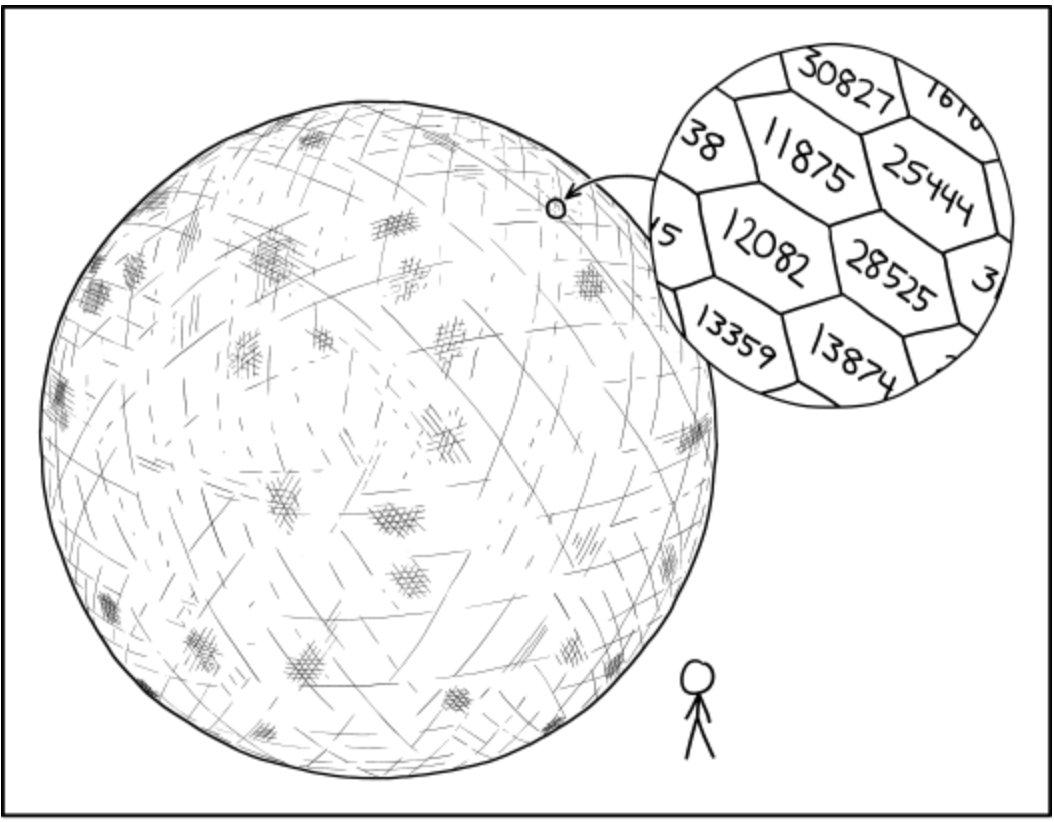
\includegraphics[width=0.5\linewidth]{xkcd/d65536.png}
    \caption{\textbf{\href{https://www.explainxkcd.com/wiki/index.php/2626:_d65536}{2626: d65536}}}
\end{figure}
